% !TEX root = ../main.tex
\subsubsection{Alignment Effect}
\label{14.11::alignment_effect}

    \begin{figure}[b!]
        \frame{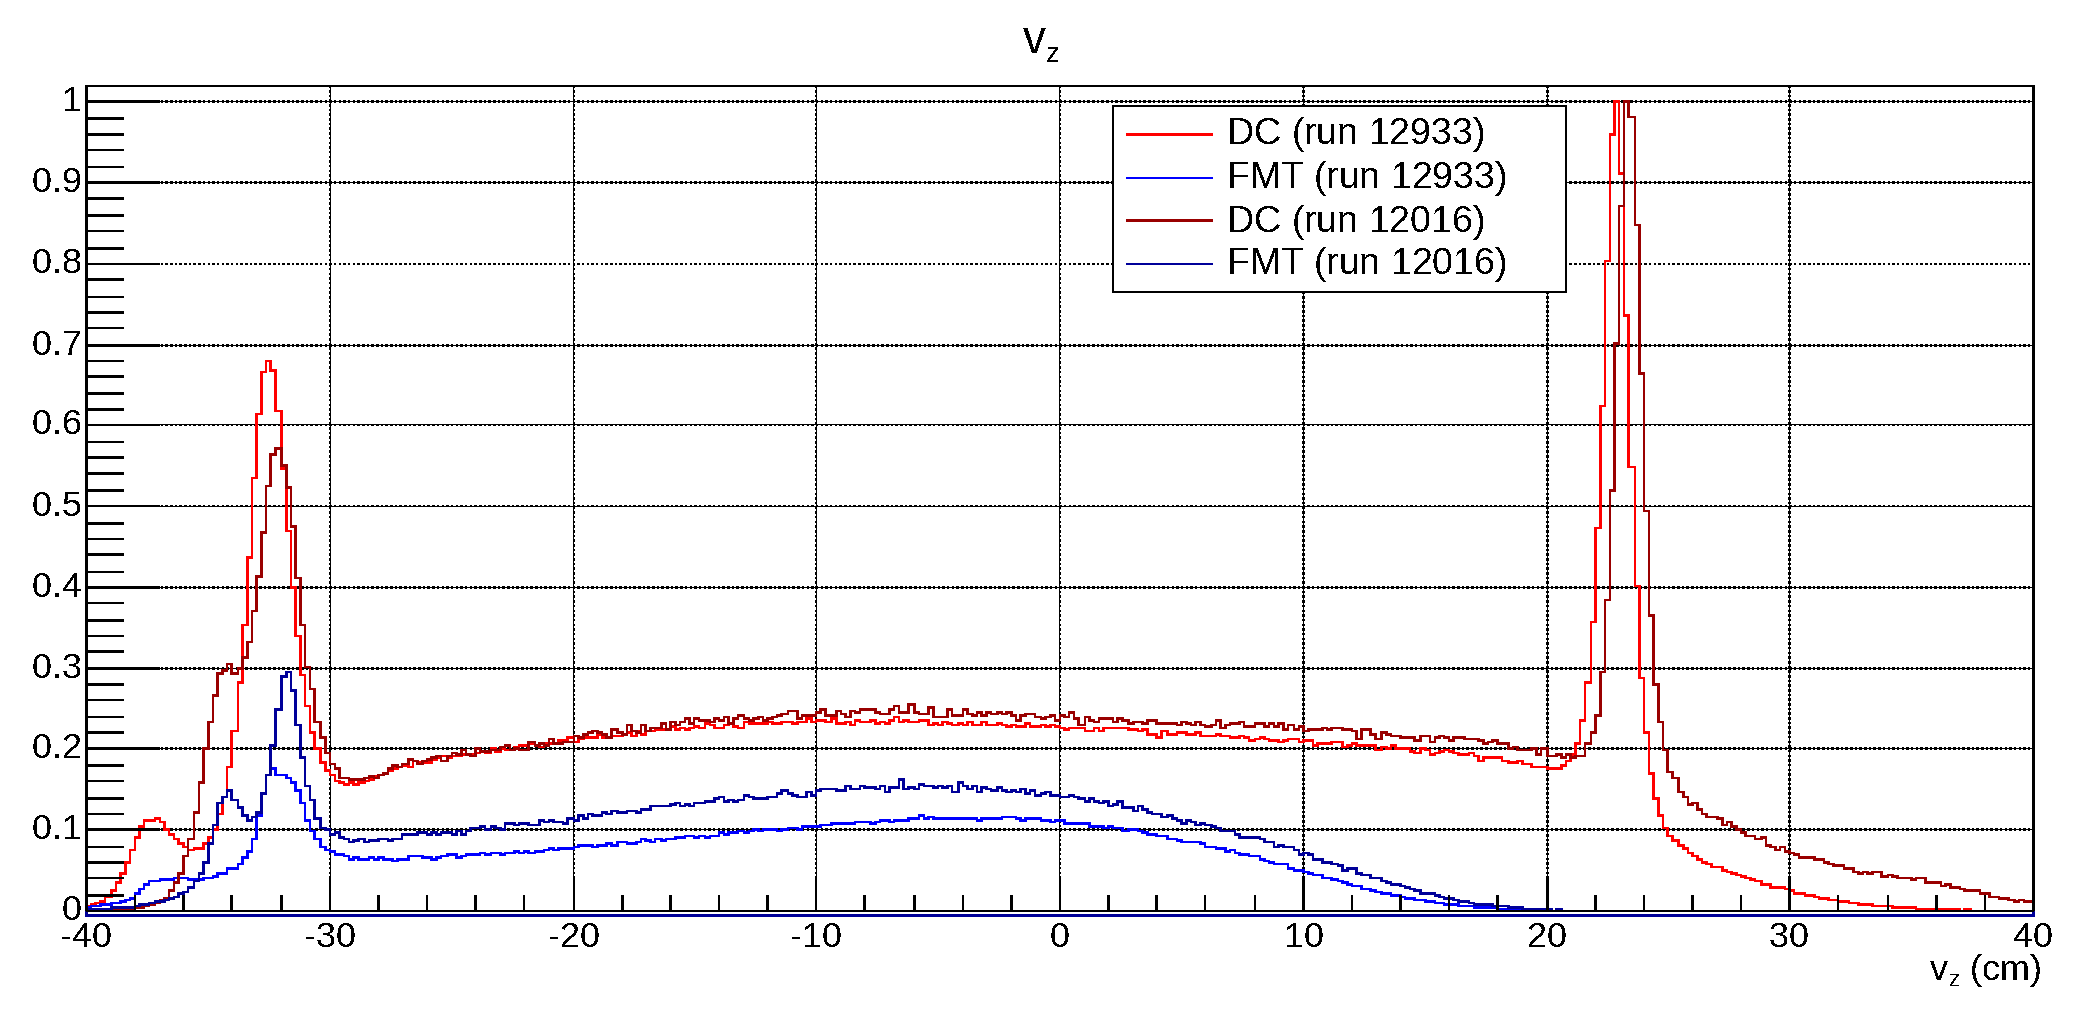
\includegraphics[width=\textwidth]{11vz_seasons.pdf}}
        \caption[$v_z$ for DC and FMT for runs 12933 and 12016]
        {$v_z$ for DC (in red) and FMT (in blue).
        Runs 12933 (Summer 2020) and 12016 (Spring 2020).}
        \floatfoot{Source: Own elaboration, using the \href{https://github.com/bleaktwig/clas12-rge-analysis}{clas12-rge-analysis} software.}
        \label{fig::14.11::vz_seasons}
    \end{figure}

    % Introduction: The problem.
    The data from the RG-F experiment is divided based on the season in which the runs take place, namely Spring 2020 and Summer 2020.
    According to the run group's guidelines, it is recommended to use Summer data as it has undergone more calibration compared to the Spring data.
    However, the calibration work conducted so far does not include the FMT detector, resulting in a significant misalignment effect.

    % Cause of the problem.
    Through simple visual inspection, two distinct peaks can be clearly observed between $z = -36$ cm and $z = -30$ cm in Figure \ref{fig::12.41::dc_vs_fmt_vz_11983}.
    The leftmost peak corresponds to the scattering chamber window, while the second peak corresponds to the RG-F target window.
    Both peaks appear flatter in the lines corresponding to run 12933 in Figure \ref{fig::14.11::vz_seasons}.
    As discussed in Section \ref{12::fmt_alignment_and_reconstruction}, this issue arises due to the lack of correction for FMT misalignments.

    % Solution.
    The simplest solution is to utilise Spring data.
    Although more calibration work has been performed on the Summer data, it mainly pertains to the CD, which is not used in this analysis.
    In the lines corresponding to run 12016 (Spring 2020) in Figure \ref{fig::14.11::vz_seasons}, we can see that both peaks are sharper.
    This indicates that the misalignment issue has been appropriately addressed in that particular run.
